\section{THGEM-based sampling elements for DHCAL}
\subsection{Introduction}
Digital Hadronic Calorimetry (DHCAL) for future experiments (e.g. ILC-SiD) requires robust thin sampling elements with high detection efficiency at low pad multiplicity. The large detection area foreseen requires cost-effective solutions.
In the past two years, a Weizmann-Aveiro-Coimbra team has shown that sampling elements based on Thick Gaseous Electron Multipliers (THGEM)~\cite{Chechik2004303} could meet DHCAL requirements. The THGEM concept has evolved from a cascade of double-sided electrodes coupled to a pad-anode through an induction gap~\cite{1748-0221-7-05-C05011}, to thinner single-sided WELL detectors - coupled to the pads with and without resistive films~\cite{1748-0221-9-04-P04011,1748-0221-8-07-P07017}.
The most recent and presently leading candidate is the Resistive Plate WELL (RPWELL). It was tested extensively in the laboratory~\cite{1748-0221-8-11-P11004,1748-0221-8-12-C12012} and at muon and high-rate pion beams at CERN-SPS. This very thin single-stage detector yielded a discharge-free operation in different gas mixtures, including Ne- and Ar-based ones, providing high detection efficiency at low pad multiplicity.

\subsubsection{The Resistive Plate WELL}
The Resistive Plate WELL (RPWELL) is a single-sided THGEM (with copper clad on one side only), coupled to the readout pads through a material sheet with high bulk resistivity (see Figure~\ref{fig:Calorimeter:THGEM:rpwell}). Materials with bulk resistivity in the $\unit[10^9]{\Omega cm}$ scale prevent significant gain-, and hence efficiency drops, at high particle flux~\cite{1748-0221-8-11-P11004}.
\begin{figure}
	\centering
	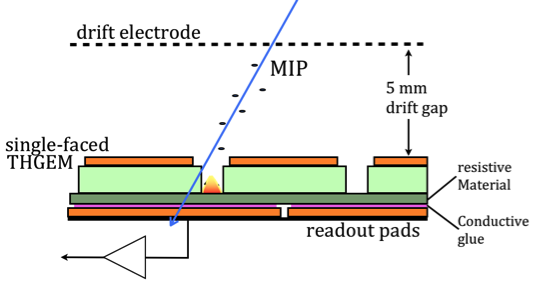
\includegraphics[width=.5\textwidth]{Calorimeter/THGEM/rpwell.png}
	\caption{The RPWELL configuration with a resistive anode and a readout electrode. The WELL, a single-faced THGEM, is coupled to a readout anode (e.g. with strips or pads) via a resistive plate.}
	\label{fig:Calorimeter:THGEM:rpwell}
\end{figure}
\subsection{Recent Milestones}
Small ($\unit[10\times 10]{cm^2}$) and medium size ($\unit[30\times 30]{cm^2}$) RPWELL detector prototypes were built and tested in the laboratory and at the CERN-SPS. The \unit[0.8]{mm} thick WELL electrodes were coupled to $\unit[1\times 1]{cm^2}$ copper pads through \unit[0.4]{mm} thick Semitron ESD225 resistive polymer ($\approx \unit[10^9]{\Omega cm}$ bulk resistivity). With a \unit[5]{mm} drift gap the sampling element had a total thickness of \unit[6.2]{mm} (excluding readout electronics – here SRS-APV~\cite{1748-0221-8-03-C03015,French2001359}).
The detection efficiency as a function of pad multiplicity (with low rate muons) is shown for the two prototypes in Figure~\ref{fig:Calorimeter:THGEM:efficiencyVSMultiplicity}. Both detectors reached high detection efficiency at low pad multiplicity when operated in our traditional Ne/5\%\ce{CH4} (Figure~\ref{fig:Calorimeter:THGEM:efficiencyVSMultiplicity} left; operation voltage, V, in the range $800-\unit[930]{V}$) and in the cost-effective Ar/5\%\ce{CH4} (Figure~\ref{fig:Calorimeter:THGEM:efficiencyVSMultiplicity} right; V in the range $1500-\unit[1720]{V}$) gas mixtures.
\begin{figure}
	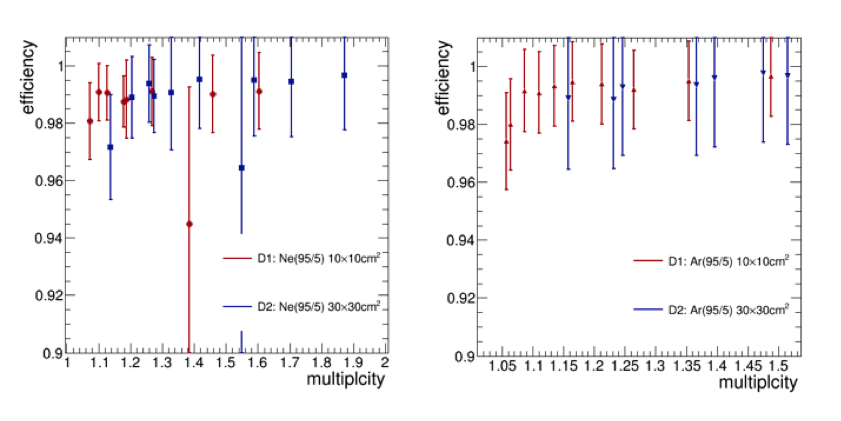
\includegraphics[width=.9\textwidth]{Calorimeter/THGEM/efficiencyVSMultiplicity.png}
	\caption{Efficiency as a function of the average pad multiplicity measured with the $\unit[10\times 10]{cm^2}$ and $\unit[30\times 30]{cm^2}$ detectors in muon beam. Left: Ne/5\%\ce{CH4} gas mixture. Right: Ar/5\%\ce{CH4} gas mixture}
	\label{fig:Calorimeter:THGEM:efficiencyVSMultiplicity}
\end{figure}
\begin{figure}
	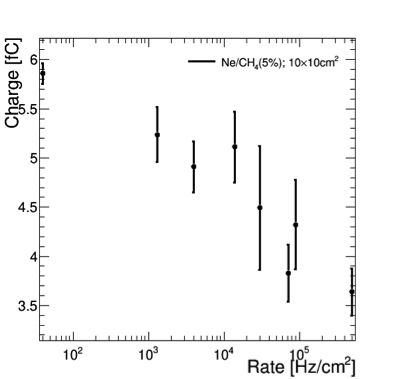
\includegraphics[width=.9\textwidth]{Calorimeter/THGEM/charge_vs_rate.png}
	\caption{The charge (estimated from the spectra most probable value) as a function of the incoming particle flux.  All the measurements were conducted at Ne/5\%\ce{CH4} gas mixture at the same operation voltage of \unit[880]{V}. A pion beam was used to generate the high incoming fluxes.}
	\label{fig:Calorimeter:THGEM:chargeVsRate}
\end{figure}
Figure~\ref{fig:Calorimeter:THGEM:chargeVsRate} shows the measured gain as a function of the particle flux; the same operation voltage of \unit[880]{V} was maintained throughout the measurements (with low rate muons as well as high rate pions). A moderate gain-drop of $\approx 30\%$ was measured while the flux was increased by 3 orders of magnitude (from 50 to $\unit[10^5]{Hz/cm^2}$). It resulted in negligible efficiency drop, since the pulse-over-threshold was sufficiently high.
Most importantly, during the two weeks of in-beam operation (which included also long time operation under high rate, $\unit[10^5]{Hz/cm^2}$, pion beam), with both Ne-based and Ar-based gas mixtures, the small prototype was completely discharge-free. The resulting discharge probability is therefore below $10^{-8}$. Occasional discharges occurring in the medium-size prototypes were traced to be associated with defects in some support pins within the active area; these can be avoided in the next prototypes.
The RPWELL laboratory and test-beam results are the subject of two articles in preparation.


\subsection{Engineering Challenges}
The novel design of a large RPWELL detector prototype (without the present support pins) is completed. Assembly and tests are foreseen in the coming year. Upon success, we are confident that future chambers could be fully industrially produced.
We are currently investigating, with industry, alternative materials and production technologies of THGEM electrodes; similarly, we are considering different resistive-plate materials, with of appropriate bulk resistivity.

\subsection{Future Plans}
As mentioned earlier, in the forthcoming year we intend to build a new medium-size detector prototype, to be followed by a prior to our square-meter one. Both prototypes will be tested in the laboratory and in muon and pion beams (CERN).
We foresee investigating the properties of several RPWELL layers in a fully-equipped DHCAL prototype; in particular their performance in measuring Hadronic showers.

\subsection{Applications Outside of Linear Colliders}
So far, our studies of THGEM-based detectors, particularly the RPWELL, have yielded a cost-effective, single-stage completely stable device, with wide dynamic range. The RPWELL concept is suitable for a variety of applications that do not require very high spatial and energy resolutions. Current examples are CsI-coated multipliers for UV-photon imaging in RICH detectors; cryogenic gaseous photomultipliers for recording scintillation-light in noble-liquid detectors, developed for future dark-matter and neutrino experiments, medical imaging and in combined neutron/gamma inspection systems; fast-neutron detectors with dedicated converter-foils and Muon tomography inspection systems for the detection of hazardous materials in cargo.
